\chapter{Diseño}

Necesidad de un nuevo sistema de control para el robot scorbot


\section{Controladores}

\label{cap3_controladores}

FUncion general y perifericos especificos

\subsection{Microcontrolador}

El microcontrolador escogido corresponde al XMC4800 de Infineon Technologies AG, 


\begin{figure}[ht]
  \centering
  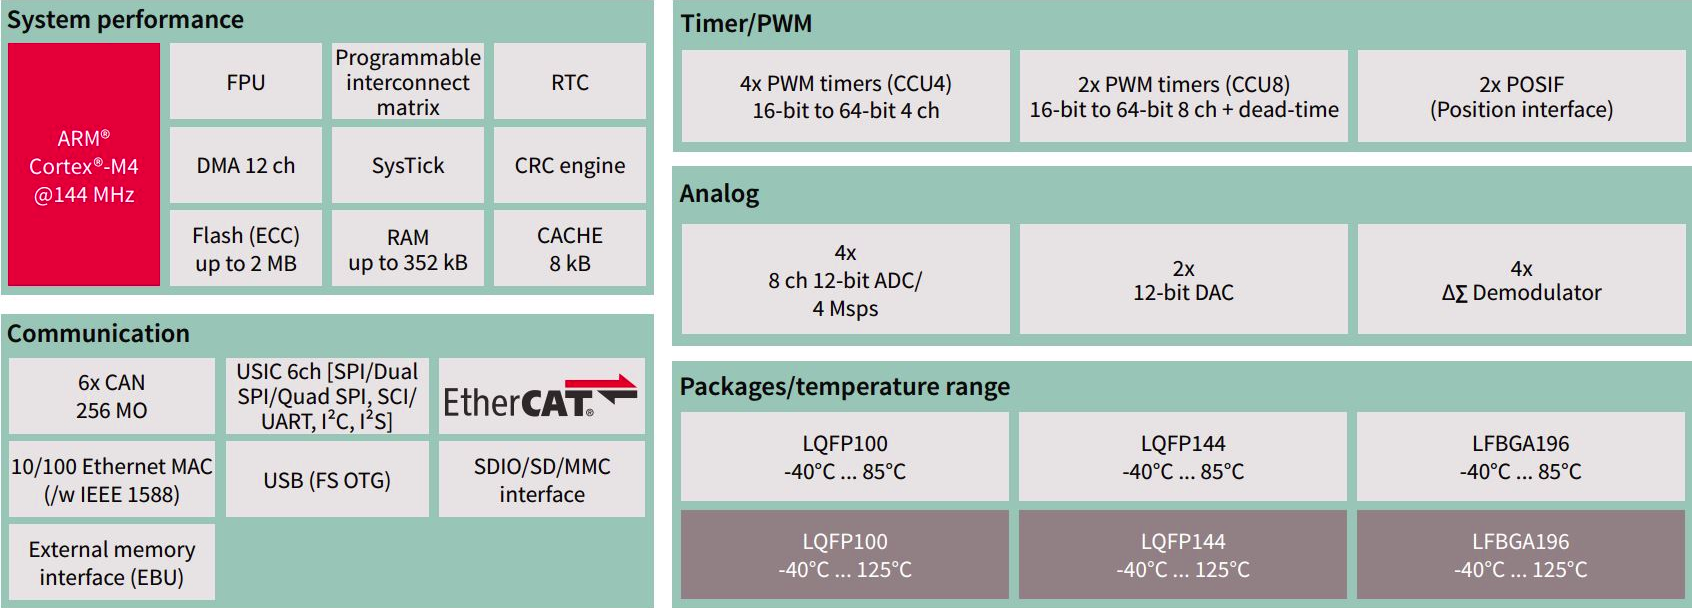
\includegraphics[scale=.2]{img/cap3/xmc4800_data}
  \caption{Carácteristicas del microcontrolador XMC4800. MO: Message Objects, Msps: Mega samples per second.}
  \label{cap3_xmc4800_data}
\end{figure}

\subsection{Puente H}

Funciones especificas

\section{Integración de hardware}

Esquematico y componentes

\subsubsection{PCB}

Placa PCB

\section{Bus de campo}

Conexión

\subsection{Uso de librerías de Ethercat}

SOEM
Flanders Mechatronics Technology Centre has decided to release their EtherCAT PR2
Ig gmbh

